\documentclass[11pt,a4paper]{article}
\usepackage[utf8]{inputenc}
\usepackage[T1]{fontenc}
\usepackage{amsmath,amsfonts,amssymb}
\usepackage{graphicx}
\usepackage{tikz}
\usetikzlibrary{shapes,arrows,positioning,calc,decorations.pathreplacing}
\usepackage{hyperref}
\usepackage{geometry}
\geometry{margin=1in}
\usepackage{listings}
\usepackage{xcolor}
\usepackage{float}

\title{ResNet for Doodle Recognition: Understanding Deep Residual Networks}
\author{Doodle Recognition Project}
\date{\today}

\begin{document}

\maketitle

\tableofcontents
\newpage

\section{Introduction}

This document explains how Machine Learning models, specifically Residual Networks (ResNet), work and how they are applied to recognize doodles from the QuickDraw dataset. The implementation uses ResNet18 with transfer learning, achieving high accuracy in classifying hand-drawn sketches across 340 different categories.

\section{Fundamentals of Doodle Recognition}

Before diving into ResNet, it is essential to understand how a machine "sees" and recognizes a doodle.

\subsection{Images as Numbers}
To a computer, a doodle is not a sketch but a grid of numbers (pixels). A $160 \times 160$ pixel grayscale image is represented as a matrix of values ranging from 0 (black) to 255 (white).
\begin{itemize}
    \item \textbf{Input}: $160 \times 160$ matrix of integers.
    \item \textbf{Goal}: Map this matrix to one of 340 categories (e.g., "cat", "airplane").
\end{itemize}

\subsection{Feature Extraction}
A machine learning model does not look at the image holistically like a human. Instead, it extracts \textbf{features}:
\begin{enumerate}
    \item \textbf{Low-level features}: Detecting horizontal lines, vertical lines, and curves.
    \item \textbf{Mid-level features}: Combining lines to form shapes (circles, squares).
    \item \textbf{High-level features}: Assembling shapes into objects (ears, wheels).
\end{enumerate}

\subsection{Classification}
The model assigns a probability to each category based on the extracted features. For example, if the model detects "pointed ears" and "whiskers", it increases the probability for "cat".

\section{What is ResNet?}

ResNet (Residual Network) is a deep convolutional neural network architecture introduced by He et al. in 2015. The key innovation of ResNet is the introduction of \textbf{residual connections} (also called skip connections), which allow the network to learn identity mappings and solve the problem of vanishing gradients in very deep networks.

\subsection{The Problem with Deep Networks}

Traditional deep neural networks face a fundamental problem: as networks get deeper, training becomes more difficult. This is due to:

\begin{itemize}
    \item \textbf{Vanishing Gradients}: Gradients become exponentially small as they propagate backward through many layers
    \item \textbf{Degradation Problem}: Deeper networks often perform worse than shallower ones, even when the deeper network can represent the same functions
\end{itemize}

\subsection{The ResNet Solution: Residual Connections}

ResNet solves these problems by introducing residual blocks. Instead of learning the desired mapping $H(x)$ directly, ResNet learns the \textbf{residual} (difference) $F(x) = H(x) - x$. The output is then computed as:

\begin{equation}
H(x) = F(x) + x
\end{equation}

This simple addition allows the network to:
\begin{itemize}
    \item Learn identity mappings easily (by setting $F(x) = 0$)
    \item Preserve gradients during backpropagation
    \item Train very deep networks (ResNet can have 50, 101, or even 152 layers)
\end{itemize}

\section{ResNet Architecture}

\subsection{Residual Block Structure}

A residual block consists of two main paths:

\begin{enumerate}
    \item \textbf{Main Path}: Convolutional layers that learn the residual $F(x)$
    \item \textbf{Skip Connection}: Direct connection that adds the input $x$ to the output
\end{enumerate}

\begin{figure}[H]
\centering
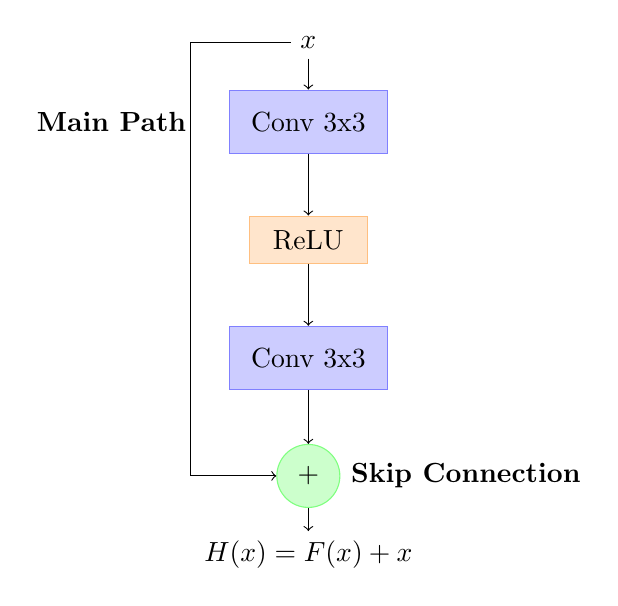
\begin{tikzpicture}[
    node distance=1.5cm,
    conv/.style={rectangle, draw=blue!50, fill=blue!20, minimum width=2cm, minimum height=0.8cm},
    add/.style={circle, draw=green!50, fill=green!20, minimum size=0.8cm},
    relu/.style={rectangle, draw=orange!50, fill=orange!20, minimum width=1.5cm, minimum height=0.6cm}
]

% Input
\node (input) {$x$};

% Main path - first conv
\node[conv, below of=input, node distance=1cm] (conv1) {Conv 3x3};
\node[relu, below of=conv1] (relu1) {ReLU};
\node[conv, below of=relu1] (conv2) {Conv 3x3};

% Skip connection
\node[add, below of=conv2, node distance=1.5cm] (add) {$+$};

% Output
\node[below of=add, node distance=1cm] (output) {$H(x) = F(x) + x$};

% Arrows - main path
\draw[->] (input) -- (conv1);
\draw[->] (conv1) -- (relu1);
\draw[->] (relu1) -- (conv2);
\draw[->] (conv2) -- (add);

% Skip connection arrow
\draw[->] (input) -| ($(add) + (-1.5,0)$) |- (add);

% Output arrow
\draw[->] (add) -- (output);

% Labels
\node[left of=conv1, node distance=2.5cm] {\textbf{Main Path}};
\node[right of=add, node distance=2cm] {\textbf{Skip Connection}};

\end{tikzpicture}
\caption{Basic Residual Block Structure}
\label{fig:residual_block}
\end{figure}

\subsection{ResNet18 Architecture}

ResNet18 is a variant with 18 layers. The architecture used in our doodle recognition model consists of:

\begin{itemize}
    \item \textbf{Initial Convolution}: 7x7 conv, stride 2 (reduces spatial dimensions)
    \item \textbf{Max Pooling}: 3x3, stride 2
    \item \textbf{4 Residual Blocks}: Each containing 2 convolutional layers
    \begin{itemize}
        \item Block 1: 64 channels, 2 layers
        \item Block 2: 128 channels, 2 layers
        \item Block 3: 256 channels, 2 layers
        \item Block 4: 512 channels, 2 layers
    \end{itemize}
    \item \textbf{Global Average Pooling}: Reduces spatial dimensions to 1x1
    \item \textbf{Fully Connected Layer}: Maps to number of classes
\end{itemize}

\begin{figure}[H]
\centering
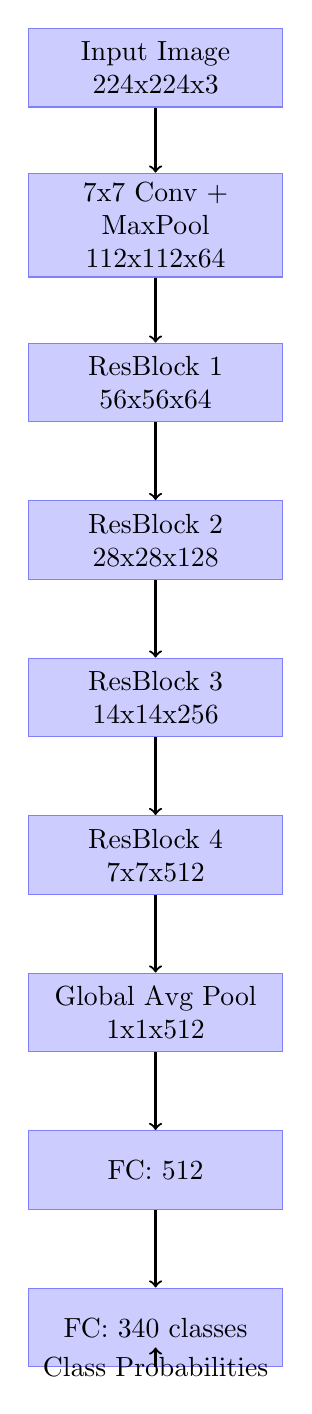
\begin{tikzpicture}[
    node distance=2.0cm,
    block/.style={rectangle, draw=blue!50, fill=blue!20, minimum width=3cm, minimum height=1cm, text centered},
    arrow/.style={->, thick}
]

% Input
\node[block, text width=3cm, align=center] (input) {Input Image\\224x224x3};

% Initial conv
\node[block, text width=3cm, align=center, below of=input] (init) {7x7 Conv + MaxPool\\112x112x64};

% Res blocks
\node[block, text width=3cm, align=center, below of=init] (res1) {ResBlock 1\\56x56x64};
\node[block, text width=3cm, align=center, below of=res1] (res2) {ResBlock 2\\28x28x128};
\node[block, text width=3cm, align=center, below of=res2] (res3) {ResBlock 3\\14x14x256};
\node[block, text width=3cm, align=center, below of=res3] (res4) {ResBlock 4\\7x7x512};

% Global pooling
\node[block, text width=3cm, align=center, below of=res4] (pool) {Global Avg Pool\\1x1x512};

% FC layers
\node[block, text width=3cm, align=center, below of=pool] (fc1) {FC: 512};
\node[block, text width=3cm, align=center, below of=fc1] (fc2) {FC: 340 classes};

% Output
\node[below of=fc2, node distance=0.5cm] (output) {Class Probabilities};

% Arrows
\draw[arrow] (input) -- (init);
\draw[arrow] (init) -- (res1);
\draw[arrow] (res1) -- (res2);
\draw[arrow] (res2) -- (res3);
\draw[arrow] (res3) -- (res4);
\draw[arrow] (res4) -- (pool);
\draw[arrow] (pool) -- (fc1);
\draw[arrow] (fc1) -- (fc2);
\draw[arrow] (fc2) -- (output);

\end{tikzpicture}
\caption{ResNet18 Architecture Overview}
\label{fig:resnet18}
\end{figure}

\section{How ResNet Recognizes Doodles}

\subsection{Feature Hierarchy}

ResNet learns a hierarchical representation of features:

\begin{enumerate}
    \item \textbf{Early Layers}: Detect low-level features (edges, curves, basic shapes)
    \item \textbf{Middle Layers}: Combine features into more complex patterns (shapes, contours)
    \item \textbf{Late Layers}: Recognize high-level concepts (objects, categories)
\end{enumerate}

For doodle recognition, this means:
\begin{itemize}
    \item Layer 1-2: Detects strokes, lines, curves
    \item Layer 3-4: Recognizes shapes (circles, rectangles, triangles)
    \item Layer 5-6: Identifies object parts (wheels, wings, faces)
    \item Layer 7-8: Classifies complete objects (cat, airplane, car)
\end{itemize}

\subsection{Transfer Learning Approach}

Our implementation uses \textbf{transfer learning} with ImageNet pre-trained weights:

\begin{enumerate}
    \item \textbf{Pre-trained Backbone}: ResNet18 trained on ImageNet (1.2M images, 1000 classes)
    \item \textbf{Custom Classifier}: Replace final layer for 340 doodle categories
    \item \textbf{Two-Stage Training}:
    \begin{itemize}
        \item Stage 1: Freeze backbone, train only classifier (10 epochs)
        \item Stage 2: Unfreeze backbone, fine-tune everything (30 epochs)
    \end{itemize}
\end{enumerate}

\begin{figure}[H]
\centering
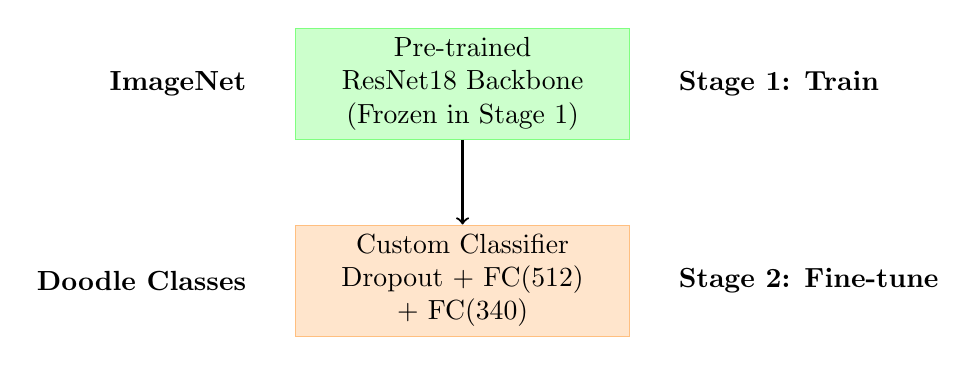
\begin{tikzpicture}[
    node distance=2.5cm,
    pretrained/.style={rectangle, draw=green!50, fill=green!20, minimum width=4cm, minimum height=1cm},
    custom/.style={rectangle, draw=orange!50, fill=orange!20, minimum width=4cm, minimum height=1cm},
    arrow/.style={->, thick}
]

% Pre-trained part
\node[pretrained, text width=4cm, align=center] (backbone) {Pre-trained ResNet18 Backbone\\(Frozen in Stage 1)};

% Custom part
\node[custom, text width=4cm, align=center, below of=backbone] (classifier) {Custom Classifier\\Dropout + FC(512) + FC(340)};

% Labels - placed further away to avoid overlap
\node[left=0.5cm of backbone] (imagenet) {\textbf{ImageNet}};
\node[left=0.5cm of classifier] (doodle) {\textbf{Doodle Classes}};

% Arrow
\draw[arrow] (backbone) -- (classifier);

% Stage labels - placed further away
\node[right=0.5cm of backbone] (stage1) {\textbf{Stage 1: Train}};
\node[right=0.5cm of classifier] (stage2) {\textbf{Stage 2: Fine-tune}};

\end{tikzpicture}
\caption{Transfer Learning Architecture}
\label{fig:transfer_learning}
\end{figure}

\subsection{Why Transfer Learning Works}

Transfer learning is effective for doodle recognition because:

\begin{itemize}
    \item \textbf{Feature Reusability}: Low-level features (edges, textures) are similar across image types
    \item \textbf{Data Efficiency}: Requires less training data than training from scratch
    \item \textbf{Faster Training}: Pre-trained weights provide good initialization
    \item \textbf{Better Generalization}: Leverages knowledge from diverse ImageNet dataset
\end{itemize}

\section{Visual Example: Predicting a "Cat" Doodle}

Let's trace the prediction process for a real example from the dataset: \texttt{cat/4503626191994880.png}.

\subsection{Step 1: Input Image}

Below is the actual doodle image from the QuickDraw dataset that we will analyze:

\begin{figure}[H]
\centering
\fbox{\includegraphics[width=4cm]{cat_sample.png}}
\caption{Input: A cat doodle from the QuickDraw dataset (\texttt{cat/4503626191994880.png})}
\label{fig:cat_input}
\end{figure}

To the model, this image is a $28 \times 28$ grid of pixel values (0-255), which is resized to $160 \times 160$ before being fed into ResNet18.

\subsection{Step 2: Convolution - How Kernels Detect Features}

The first layers of ResNet apply \textbf{convolutional filters} (kernels) to detect basic features like edges. Here's how a vertical edge detector works:

\begin{figure}[H]
\centering
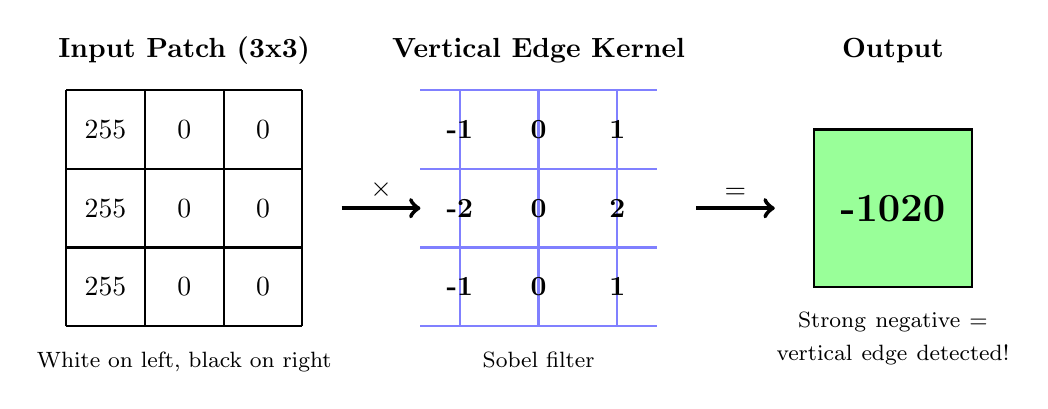
\begin{tikzpicture}

% === LEFT: Input patch ===
\node[font=\bfseries] at (1.5, 4.5) {Input Patch (3x3)};
\draw[step=1cm, black, thick] (0,1) grid (3,4);
% Fill with example pixel values (simplified)
\node at (0.5, 3.5) {255};
\node at (1.5, 3.5) {0};
\node at (2.5, 3.5) {0};
\node at (0.5, 2.5) {255};
\node at (1.5, 2.5) {0};
\node at (2.5, 2.5) {0};
\node at (0.5, 1.5) {255};
\node at (1.5, 1.5) {0};
\node at (2.5, 1.5) {0};
\node[below] at (1.5, 0.8) {\footnotesize White on left, black on right};

% === MIDDLE: Kernel ===
\draw[->, ultra thick] (3.5, 2.5) -- (4.5, 2.5);
\node[above] at (4, 2.5) {$\times$};

\node[font=\bfseries] at (6, 4.5) {Vertical Edge Kernel};
\draw[step=1cm, blue!50, thick, fill=blue!10] (4.5,1) grid (7.5,4);
\node at (5, 3.5) {\textbf{-1}};
\node at (6, 3.5) {\textbf{0}};
\node at (7, 3.5) {\textbf{1}};
\node at (5, 2.5) {\textbf{-2}};
\node at (6, 2.5) {\textbf{0}};
\node at (7, 2.5) {\textbf{2}};
\node at (5, 1.5) {\textbf{-1}};
\node at (6, 1.5) {\textbf{0}};
\node at (7, 1.5) {\textbf{1}};
\node[below] at (6, 0.8) {\footnotesize Sobel filter};

% === RIGHT: Output ===
\draw[->, ultra thick] (8, 2.5) -- (9, 2.5);
\node[above] at (8.5, 2.5) {$=$};

\node[font=\bfseries] at (10.5, 4.5) {Output};
\draw[thick, fill=green!40] (9.5,1.5) rectangle (11.5,3.5);
\node[font=\Large\bfseries] at (10.5, 2.5) {-1020};
\node[below, text width=3cm, align=center] at (10.5, 1.3) {\footnotesize Strong negative = vertical edge detected!};

\end{tikzpicture}
\caption{Convolution operation: The kernel slides over the image and produces high activations where edges are detected.}
\label{fig:convolution_example}
\end{figure}

\textbf{Calculation:} $(255 \times -1) + (255 \times -2) + (255 \times -1) + (0 \times 1) + (0 \times 2) + (0 \times 1) = -1020$

A large magnitude indicates a strong edge was detected at this location.

\subsection{Step 3: Feature Hierarchy Through Layers}

As the image passes through ResNet's layers, simple features combine into complex ones:

\begin{figure}[H]
\centering
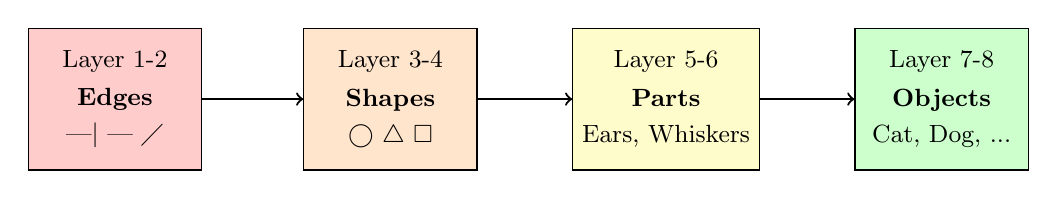
\begin{tikzpicture}[
    box/.style={rectangle, draw, minimum width=2.2cm, minimum height=1.8cm, align=center, font=\small},
    arrow/.style={->, thick}
]

% Layer boxes
\node[box, fill=red!20] (l1) at (0,0) {Layer 1-2\\[3pt]\textbf{Edges}\\[2pt]|\textbar{} --- $\diagup$};
\node[box, fill=orange!20] (l2) at (3.5,0) {Layer 3-4\\[3pt]\textbf{Shapes}\\[2pt]$\bigcirc$ $\triangle$ $\square$};
\node[box, fill=yellow!20] (l3) at (7,0) {Layer 5-6\\[3pt]\textbf{Parts}\\[2pt]Ears, Whiskers};
\node[box, fill=green!20] (l4) at (10.5,0) {Layer 7-8\\[3pt]\textbf{Objects}\\[2pt]Cat, Dog, ...};

% Arrows
\draw[arrow] (l1) -- (l2);
\draw[arrow] (l2) -- (l3);
\draw[arrow] (l3) -- (l4);

\end{tikzpicture}
\caption{Feature hierarchy: Early layers detect edges, later layers recognize complete objects.}
\label{fig:feature_hierarchy}
\end{figure}

For our cat doodle:
\begin{itemize}
    \item \textbf{Layer 1-2}: Detects vertical lines (ears), curved lines (head outline), horizontal lines (whiskers).
    \item \textbf{Layer 3-4}: Recognizes triangular shapes (pointed ears), circular shape (head).
    \item \textbf{Layer 5-6}: Identifies cat-specific features: ``pointed ears'' + ``whiskers'' + ``round face''.
    \item \textbf{Layer 7-8}: Combines all features and outputs class probabilities.
\end{itemize}

\subsection{Step 4: Final Prediction}

The model outputs a probability distribution over all 340 classes:

\begin{figure}[H]
\centering
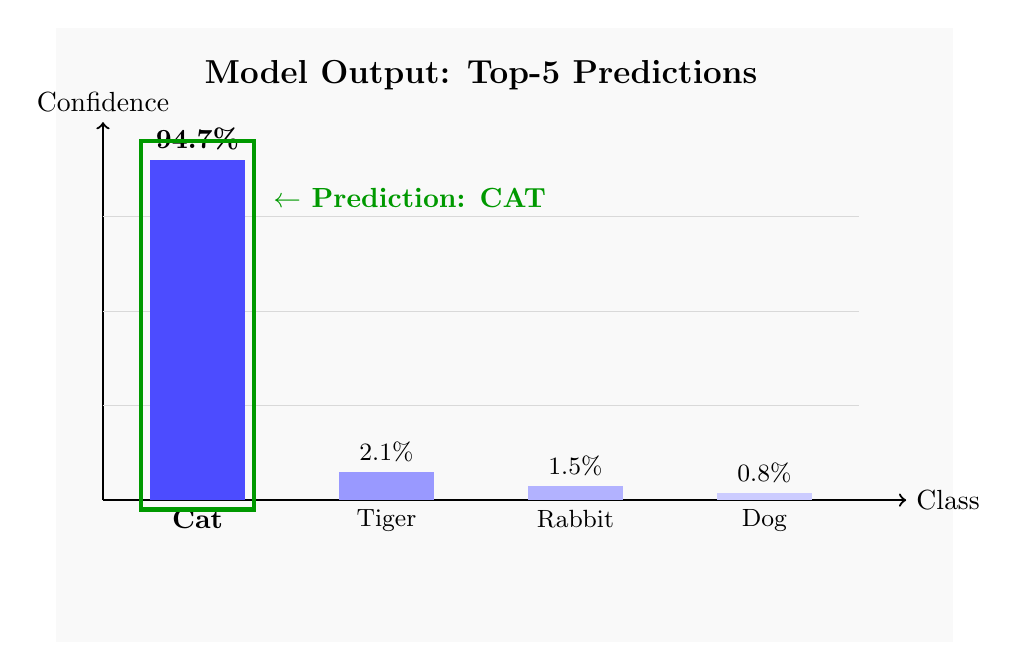
\begin{tikzpicture}[scale=1.2]
    % Background
    \fill[gray!5] (-0.5,-1.5) rectangle (9,5);
    
    % Title
    \node[font=\bfseries\large] at (4, 4.5) {Model Output: Top-5 Predictions};
    
    % Axes
    \draw[thick, ->] (0,0) -- (8.5,0) node[right] {Class};
    \draw[thick, ->] (0,0) -- (0,4) node[above] {Confidence};
    
    % Grid lines
    \foreach \y in {1,2,3} {
        \draw[gray!30] (0,\y) -- (8,\y);
    }
    
    % Bars with gradient
    \fill[blue!70] (0.5,0) rectangle (1.5, 3.6);
    \fill[blue!40] (2.5,0) rectangle (3.5, 0.3);
    \fill[blue!30] (4.5,0) rectangle (5.5, 0.15);
    \fill[blue!20] (6.5,0) rectangle (7.5, 0.08);
    
    % Percentage labels
    \node[above, font=\bfseries] at (1, 3.6) {94.7\%};
    \node[above, font=\small] at (3, 0.3) {2.1\%};
    \node[above, font=\small] at (5, 0.15) {1.5\%};
    \node[above, font=\small] at (7, 0.08) {0.8\%};
    
    % Class labels
    \node[below, font=\bfseries] at (1, 0) {Cat};
    \node[below, font=\small] at (3, 0) {Tiger};
    \node[below, font=\small] at (5, 0) {Rabbit};
    \node[below, font=\small] at (7, 0) {Dog};
    
    % Highlight winner
    \draw[green!60!black, ultra thick] (0.4, -0.1) rectangle (1.6, 3.8);
    \node[green!60!black, font=\bfseries, right] at (1.7, 3.2) {$\leftarrow$ Prediction: CAT};
    
\end{tikzpicture}
\caption{Final prediction probabilities for the cat doodle. The model correctly classifies it as ``Cat'' with 94.7\% confidence.}
\label{fig:prediction_chart}
\end{figure}

\subsection{Another Example: Airplane}

\begin{figure}[H]
\centering
\fbox{\includegraphics[width=4cm]{airplane_sample.png}}
\caption{Input: An airplane doodle from the QuickDraw dataset}
\label{fig:airplane_input}
\end{figure}

For the airplane, ResNet detects:
\begin{itemize}
    \item \textbf{Edges}: Long horizontal lines (wings), vertical line (fuselage)
    \item \textbf{Shapes}: Elongated body, triangular tail/nose
    \item \textbf{Parts}: Wing configuration, tail fin, cockpit area
    \item \textbf{Result}: Classified as ``Airplane'' with high confidence
\end{itemize}

\section{Implementation Details}

\subsection{Model Configuration}

The ResNet18 model used in the notebook has the following configuration:

\begin{itemize}
    \item \textbf{Input Size}: 160x160 pixels (resized from original doodles)
    \item \textbf{Pre-trained Weights}: ImageNet1K\_V1
    \item \textbf{Custom Classifier}:
    \begin{itemize}
        \item Dropout (0.5)
        \item Linear: 512 features
        \item BatchNorm + ReLU
        \item Dropout (0.3)
        \item Linear: 340 classes (number of doodle categories)
    \end{itemize}
    \item \textbf{Total Parameters}: 11.6M (11,614,612)
    \item \textbf{Trainable Parameters}: 438K (438,100) in Stage 1
\end{itemize}

\subsection{Training Strategy}

The two-stage training approach:

\begin{enumerate}
    \item \textbf{Stage 1} (Epochs 1-10):
    \begin{itemize}
        \item Freeze ResNet18 backbone
        \item Train only custom classifier
        \item Learning rate: 1e-3
        \item Purpose: Stabilize classifier with pre-trained features
    \end{itemize}
    
    \item \textbf{Stage 2} (Epochs 11-40):
    \begin{itemize}
        \item Unfreeze all parameters
        \item Fine-tune entire network
        \item Learning rates: Backbone 1e-4, Classifier 5e-4
        \item Purpose: Adapt features to doodle-specific patterns
    \end{itemize}
\end{enumerate}

\subsection{Data Augmentation}

To improve generalization, the following augmentations are applied:

\begin{itemize}
    \item Random crop (160x160)
    \item Random horizontal flip (50\% probability)
    \item Random rotation (±15 degrees)
    \item Random affine transformation (translation, shear, scale)
    \item Color jitter (brightness, contrast, saturation, hue)
    \item ImageNet normalization
\end{itemize}

\section{Results}

The ResNet18 model achieves:

\begin{itemize}
    \item \textbf{Test Accuracy}: 75.03\%
    \item \textbf{Top-3 Accuracy}: 90.70\%
    \item \textbf{Training Samples}: 238,000
    \item \textbf{Validation Samples}: 51,000
    \item \textbf{Test Samples}: 51,000
    \item \textbf{Number of Classes}: 340
\end{itemize}

\section{Why Residual Connections Matter}

Residual connections enable ResNet to:

\begin{enumerate}
    \item \textbf{Learn Identity Mappings}: If optimal mapping is identity, $F(x) = 0$ is easier to learn than $H(x) = x$
    \item \textbf{Preserve Gradients}: Skip connections provide direct gradient paths
    \item \textbf{Enable Deep Networks}: Can train networks with 50+ layers effectively
    \item \textbf{Improve Accuracy}: Deeper networks can learn more complex features
\end{enumerate}

Mathematically, the gradient flows through both paths:

\begin{equation}
\frac{\partial L}{\partial x} = \frac{\partial L}{\partial H} \cdot \left(1 + \frac{\partial F}{\partial x}\right)
\end{equation}

Even if $\frac{\partial F}{\partial x}$ is small, the gradient can still flow through the identity connection.

\section{Conclusion}

ResNet's residual connections solve the vanishing gradient problem, enabling training of very deep networks. When combined with transfer learning, ResNet18 provides an effective solution for doodle recognition, achieving high accuracy on the QuickDraw dataset with relatively few trainable parameters. The hierarchical feature learning and skip connections make ResNet particularly well-suited for recognizing the diverse, hand-drawn sketches in the dataset.

\section{References}

\begin{itemize}
    \item He, K., Zhang, X., Ren, S., \& Sun, J. (2016). Deep residual learning for image recognition. CVPR.
    \item QuickDraw Dataset: \url{https://github.com/googlecreativelab/quickdraw-dataset}
    \item PyTorch ResNet Implementation: \url{https://pytorch.org/vision/stable/models.html}
\end{itemize}

\end{document}

